\documentclass[oneside,final,14pt]{extreport}
\usepackage{pdfpages} % поддержка вставки страниц из pdf-файлов
\usepackage[onehalfspacing]{setspace} % 1,5 интервал
\usepackage[top=2.0cm,bottom=2.0cm,left=2.0cm,right=1.0cm]{geometry} % поля
\usepackage{lscape} % поддержка альбомной ориентации страниц
\usepackage{indentfirst} % красная строка
\setlength\parindent{1.5cm} % установка величины отступа красной строки

\usepackage{etoolbox} % позволяет добавлять произвольный код в начало любой команды, и содержит прочие подобные доп. функции для программирования
\usepackage{suffix} % позволяет легко определять команды со звёздочкой (starred version of command)
\usepackage{afterpage} % float overload fix
\usepackage{placeins} % float barrier

% Шрифты
\usepackage[cm-default]{fontspec}
\usepackage{xunicode}
\usepackage{xltxtra}
%\setromanfont[Mapping=tex-text]{Times New Roman}
\setmainfont[Mapping=tex-text]{Times New Roman}
\setsansfont{Calibri}
\setmonofont{Consolas}
\defaultfontfeatures{Scale=MatchLowercase, Mapping=tex-text} % одинаковый рост строчных букв у разных гарнитур, маппинги TeXовских лигатур вроде -- и ---
\usepackage{ulem} % поддержка подчёркиваний

% Поддержка русского языка и русскоязычных стилей
\usepackage{polyglossia}
\setmainlanguage[babelshorthands=true]{russian} % основной язык - русский
\setotherlanguage[variant=us]{english} % дополнительный язык - английский

% Формулы
\usepackage{amsmath}
\usepackage{amstext} % поддержка текста внутри формул
\usepackage{amssymb} % дополнительные символы в математических формулах
%\usepackage{icomma} % запятая в качестве десятичного разделителя
\usepackage{chngcntr} % управление нумерацией
\counterwithout{equation}{chapter} % сквозная нумерация формул
% поддержка кириллицы в формулах (не работает, хотя должно)
%\usepackage{unicode-math}
%\setmathfont[math-style=TeX]{Cambria Math}
%\usepackage[warn]{mathtext}

% Формат заголовков
\usepackage{titlesec}
\setcounter{secnumdepth}{3} % включает нумерацию subsubsection
\newcommand{\nhspacesize}{10pt}
\newcommand{\nohyphenation}{\righthyphenmin62}
\titleformat{\chapter}[hang]{\nohyphenation\sloppy\Large\bfseries}{\thechapter}{\nhspacesize}{} % righthypenmin62 - не переносить слова в названиях глав
\titleformat{\section}[hang]{\nohyphenation\sloppy\large\bfseries}{\thesection}{\nhspacesize}{}
\titleformat{\subsection}[hang]{\sloppy\normalsize\bfseries}{\thesubsection}{\nhspacesize}{}
\titleformat{\subsubsection}[hang]{\sloppy\normalsize\bfseries}{\thesubsubsection}{\nhspacesize}{}
\titlespacing*{\chapter}{\parindent}{-30pt}{*4}
\titlespacing*{\section}{\parindent}{*4}{*2}
\titlespacing*{\subsection}{\parindent}{*2}{*1}
\titlespacing*{\subsubsection}{\parindent}{*1}{*1}
%\setlength{\parskip}{1ex plus 0.5ex minus 0.2ex} % если вдруг нужен интервал между абзацами

% Новый формат заголовков - специальные разделы (реферат, вступление, заключение и т.п.)
\newcommand{\spchapterStar}[1]{
	\clearpage
	\begin{center}
		\nohyphenation{\sloppy{\textbf{\Large{#1}}}}
	\end{center}
	\par}
\newcommand{\spchapter}[1]{
	\spchapterStar{#1}
	\addcontentsline{toc}{chapter}{#1}}
\WithSuffix\newcommand\spchapter*[1]{\spchapterStar{#1}}

% Формат списков
\usepackage{enumitem}
\setlist{nolistsep} % убрать лишний интервал между элементами списка
\setlist[itemize,1]{label={–}, labelindent=\parindent, leftmargin=*} % маркированные списки: символ - короткое тире, выравнивание символа по красной строке
\AddEnumerateCounter{\asbuk}{\asbuk}{д} % последний параметр - самый широкий символ в перечислении
\setlist[enumerate,1]{label={\asbuk*}), labelindent=\parindent, leftmargin=*}
\setlist[enumerate,2]{label={\arabic*}), leftmargin=\parindent}
\setlist[description]{labelindent=\parindent, leftmargin=0pt, font=\textmd}

% Поддержка изображений
\usepackage{graphicx}
\graphicspath{{./images/chapter1/}{./images/chapter2/}{./images/chapter3/}{./images/chapter4/}} % пути к каталогам с изображениями
\usepackage{svg} % поддержка вставки векторных (SVG) изображений (из Inkscape) - команда includesvg

% Таблицы
%\usepackage{makecell}
%\usepackage{tabularx}
\usepackage{array}
\usepackage{longtable}
\usepackage{multirow}

%\newcolumntype{CL}[1]{>{\arraybackslash}m{#1}}
\newcolumntype{C}[1]{>{\centering\arraybackslash}m{#1}}
%\newcolumntype{CR}[1]{>{\raggedright\arraybackslash}m{#1}}
%\newcolumntype{TL}[1]{>{\arraybackslash}p{#1}}
%\newcolumntype{TC}[1]{>{\centering\arraybackslash}p{#1}
%\newcolumntype{TR}[1]{>{\raggedright\arraybackslash}p{#1}}
%\newcolumntype{BL}[1]{>{\arraybackslash}b{#1}}
%\newcolumntype{BC}[1]{>{\centering\arraybackslash}b{#1}}
%\newcolumntype{BR}[1]{>{\raggedright\arraybackslash}b{#1}}
%\newcommand{\ptw}[1]{#1\linewidth}

\setlength{\extrarowheight}{4pt}
%\renewcommand{\arraystretch}{1.5}
%\newcommand{\tn}{\tabularnewline}
%\newcommand{\tnhl}{\tabularnewline\hline}
%\newcommand{\tncl}[1]{\tabularnewline\cline{#1}}

% Формат рисунков и таблиц
\usepackage{caption} % подписи
\captionsetup{labelsep=endash, textformat=simple, figurename=Рисунок, tablename=Таблица, figurewithin=none, tablewithin=none} % разделитель подписи и названия - короткое тире, заголовок - название float'a и номер, имена рисунков и таблиц по ГОСТу, сквозная нумерация рисунков и таблиц
\captionsetup[figure]{position=above}
\captionsetup[table]{singlelinecheck=false, position=top, justification=raggedright}
% подписи многостраничных таблиц
\newcommand{\LTcontcaption}[1]{\captionsetup{justification=raggedleft, singlelinecheck=false,position=top,font=it}\caption*{Продолжение таблицы~\ref{#1}}}
\newcommand{\LTendcaption}[1]{\captionsetup{justification=raggedleft, singlelinecheck=false,position=top,font=it}\caption*{ Окончание таблицы~\ref{#1}}}
%\DeclareCaptionLabelFormat{continued}{#1~#2 (\textit{продолжение})}
%\captionsetup[ContinuedFloat]{labelformat=continued}
\usepackage{floatrow} % пакет для настройки размещения float'ов и их подписей
\floatsetup[table]{style=plaintop, justification=justified} % название над таблицей, таблица выровнена по ширине влево

% Библиография и библиографические ссылки
\usepackage{cite}
% Замена формата нумерации списка литературы с "[1]" на "1."
\makeatletter
\renewcommand{\@biblabel}[1]{#1.}
\makeatother
\bibliographystyle{utf8gost705u}
\gappto\captionsrussian{\renewcommand{\bibname}{Список использованных источников}}

% Оглавление
\gappto\captionsrussian{\renewcommand{\contentsname}{Содержание}}
\usepackage[subfigure,titles]{tocloft}
\renewcommand{\cftchapleader}{\bfseries\cftdotfill{\cftdotsep}} % точечки не только у глав, но и у всего остального
% расстояние от номера до названия (чтобы номер на название на заезжал)
\setlength{\cftchapnumwidth}{2em}
\setlength{\cftsecnumwidth}{3em}
\setlength{\cftsubsecnumwidth}{4em}

% Подсчёт объектов (для реферата)
\usepackage{totcount}
%\regtotcounter{figure} % рисунки
%\regtotcounter{table} % таблицы
% подсчёт приложений
\newtotcounter{appendixcount}
\usepackage{apptools}
\pretocmd{\chapter}{\IfAppendix{\addtocounter{appendixcount}{1}}{}}{}{}
% подсчёт страниц
\usepackage{lastpage}
\newcommand{\pagecount}{\pageref{LastPage}}
% подсчёт использованных источников
\newtotcounter{refcount}
\pretocmd{\bibitem}{\addtocounter{refcount}{1}}{}{}
% подсчёт рисунков и таблиц
\newtotcounter{figurecount}
\newtotcounter{tablecount}
\AfterEndEnvironment{figure}{\addtocounter{figurecount}{1}}
\AfterEndEnvironment{table}{\addtocounter{tablecount}{1}}
\AfterEndEnvironment{longtable}{\addtocounter{tablecount}{1}}

% Оформление приложений
\usepackage[title, titletoc]{appendix}
% задание своего формата заголовков для приложений
\pretocmd{\appendix}{
	\titleformat{\chapter}[display]{\nohyphenation\sloppy\normalsize\centering}{\MakeUppercase{\chaptertitlename} \thechapter}{\nhspacesize}{\bfseries}{}
	\counterwithin{equation}{chapter}
	\counterwithin{figure}{chapter}
	\counterwithin{table}{chapter}
}{}{}


\begin{document}
	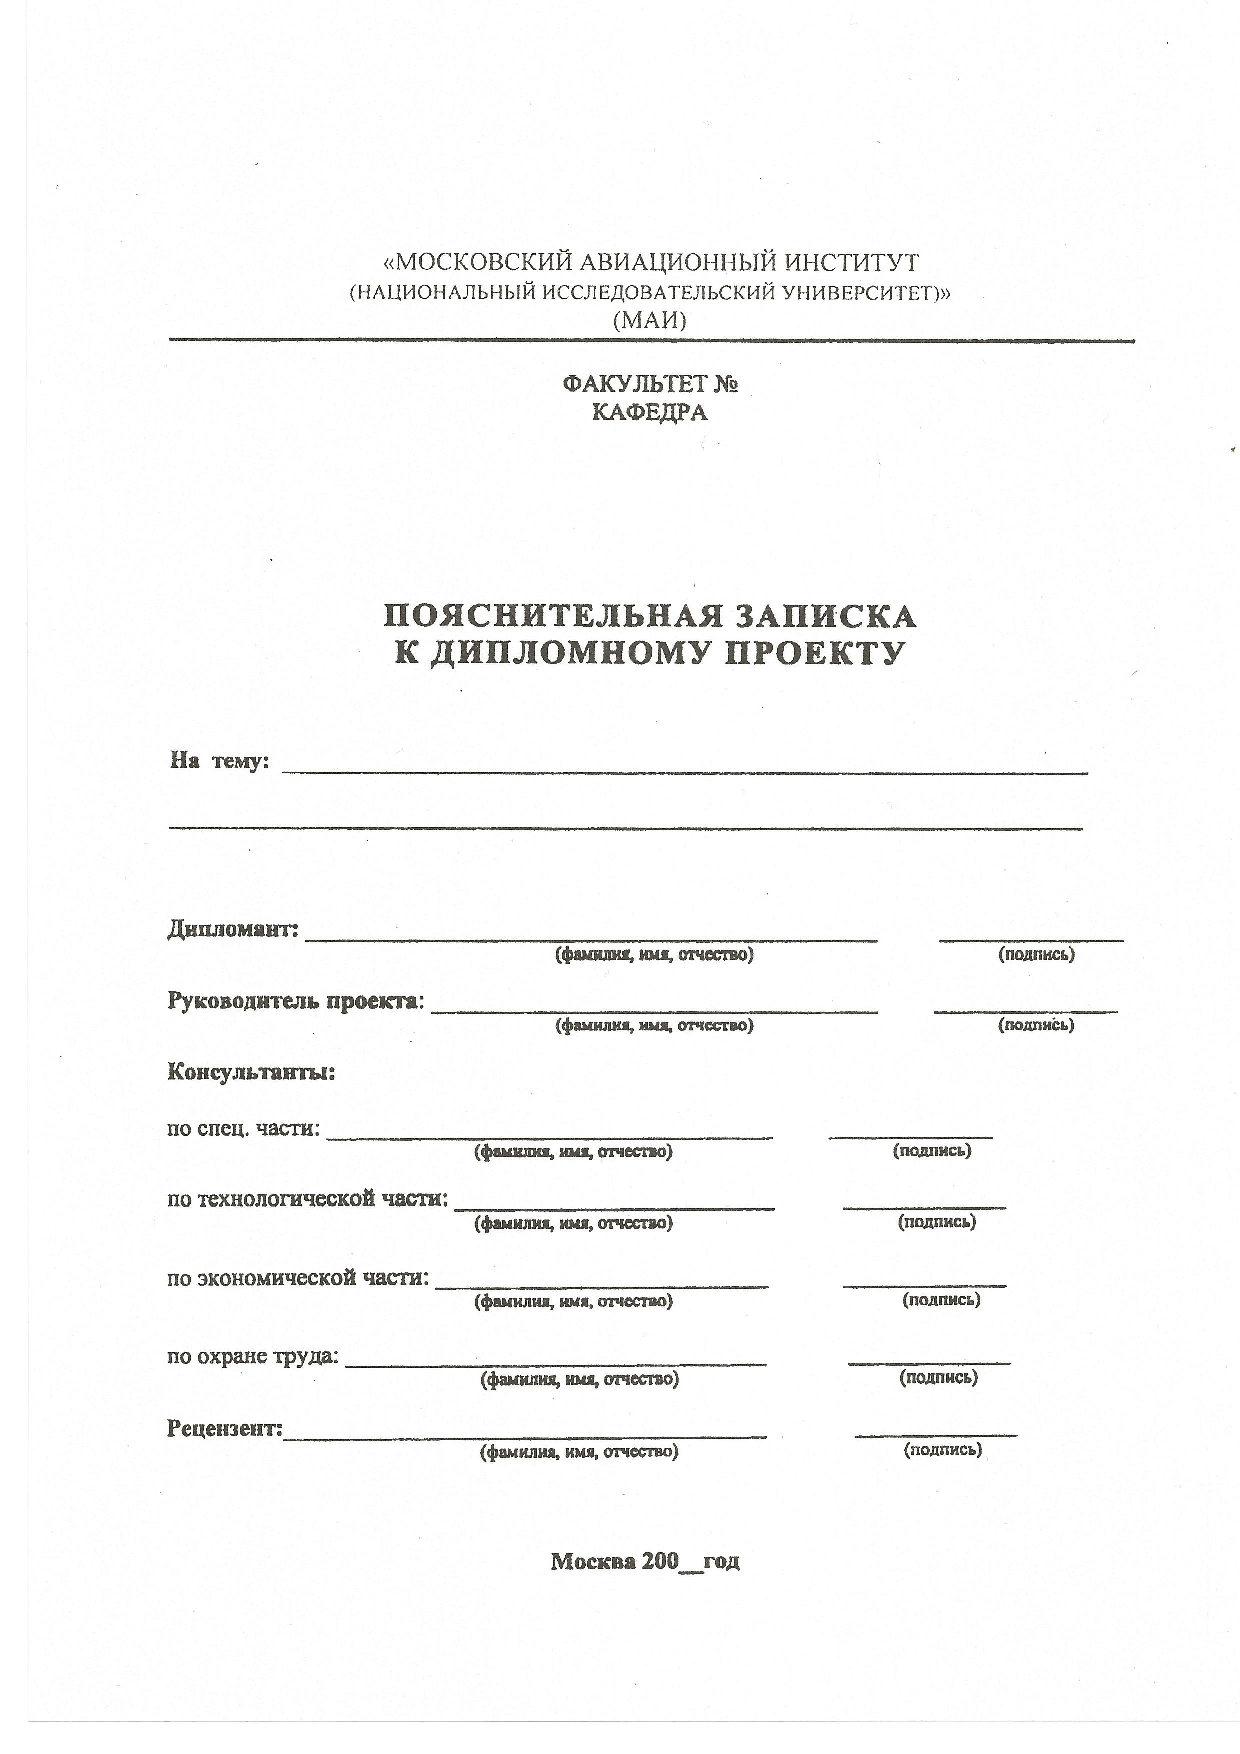
\includepdf[pages={1}]{title.pdf} % титульник
	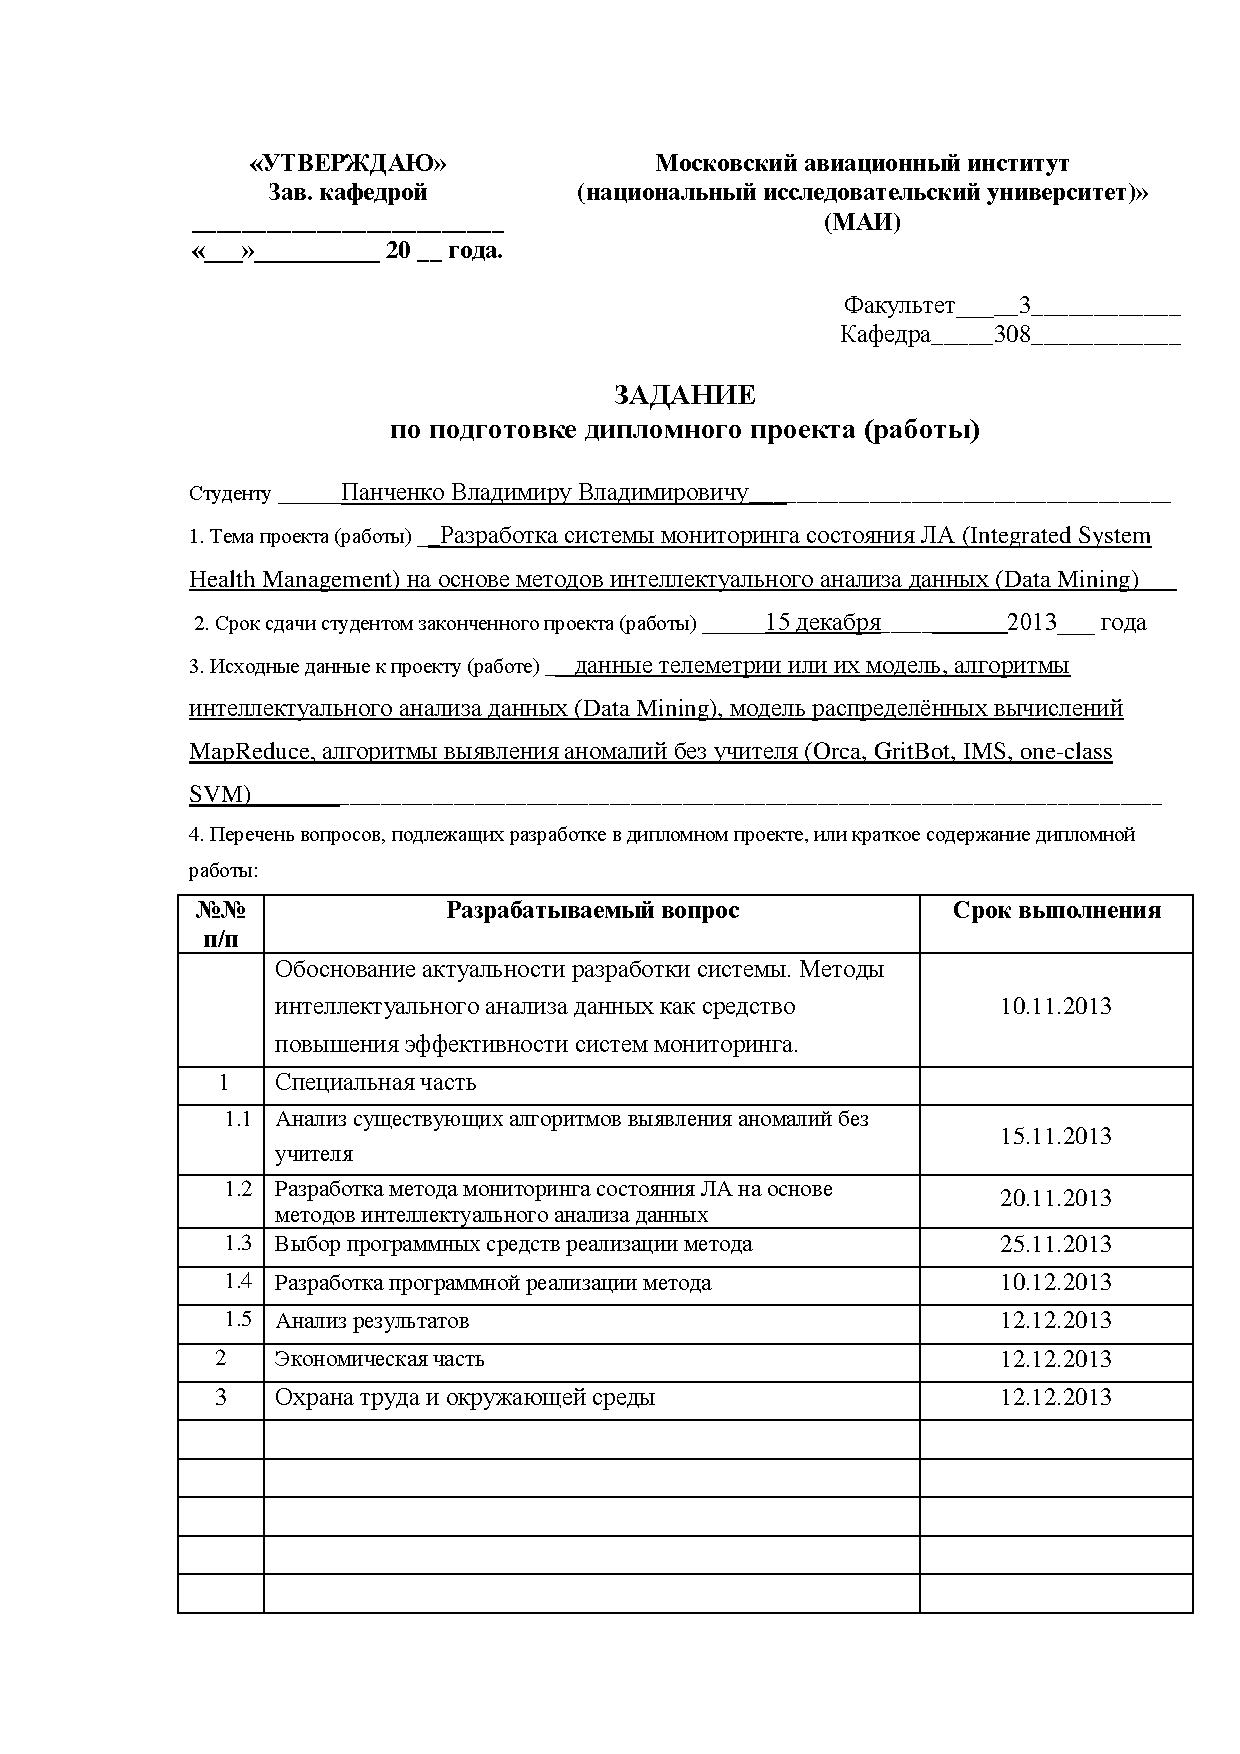
\includepdf[pages={1,2}]{assignment.pdf} % задание
	\setcounter{page}{3} % начать нумерацию страниц с №3
	\protect\spchapter*{\MakeUppercase{Реферат}}
\sloppy
{
\theauthor\ \MakeUppercase{\thethesistitle}, дипломная работа: \pagestotal~с., \figurestotal~рис., \tablestotal~табл., \bibitemstotal~ист., \appendicestotal~прил.

Ключевые слова: \MakeUppercase{\thekeywords}
}
\medskip

В данной дипломной работе разработан и реализован в виде программной системы метод мониторинга состояния ЛА на основе алгоритмов интеллектуального анализа данных (Data Mining).

Разработанный в работе метод позволяет производить контроль и диагностику состояния системы в реальном времени на основе архивных данных телеметрии при различных режимах работы, без априорных знаний о предметной области, назначении системы, её составе, конструкции. Метод относится к классу искусственного интеллекта, используя машинное обучение (обучение без учителя) для построения модели системы.

Программная реализация метода прошла тестирование, подтвердив свою эффективность с точки зрения быстродействия и достоверности контроля, позволяя своевременно обнаруживать аномалии в работе систем.

Работа имеет практическое значение в рамках деятельности научно-измерительных пунктов (НИП), где может применяться для своевременного контроля состояния ЛА и обнаружения аномалий в работе оборудования на основе данных телеметрии.
	\tableofcontents
	
	\spchapter{Введение}
Одной из ключевых проблем при эксплуатации летальных аппаратов (ЛА) является контроль и своевременная диагностика неисправностей. Подобный контроль выполняется на основе информации, поступающей с датчиков, контролирующих работу устройства. Для решения подобных задач используются системы ISHM (Integrated System Health Management) позволяющие оценить текущее и/или будущее состояние здоровья системы и интегрировать эту информацию в общую картину эксплуатационных потребностей с учётом имеющихся ресурсов~\cite{JennionsIVHM}. В ISHM состояние системы контролируется по показаниям датчиков. Прогресс в развитии микроэлектроники за последние 10--15 лет привел к тому, что датчики стали существенно дешевле, легче и меньше по размерам. Это вызвало увеличение количества используемых датчиков и рост объемов телеметрической информации. Естественно, ручная обработка больших объемов информации слишком трудоемка~–--~нужны средства автоматизации.

Традиционно системы ISHM используют одновременно несколько методов диагностики, в частности~\cite{FaultDetectionByMiningAssocRules}:
\begin{itemize}
	\item проверку выхода значения параметра за установленные пределы;
	\item экспертную систему, содержащую набор правил, описывающих нормальное поведение системы (rule-based);
	\item математическую модель, описывающую требуемое поведение системы (model-based).
\end{itemize}

Общий принцип у традиционных алгоритмов примерно один и тот же. Вначале эксперты задают модель поведения системы, представляющую набор правил, характеризующих поведение системы. В процессе работы системы поступающие телеметрические данные проверяются на соответствие модели. Если поведение данных начинает отклоняться от модели, то оператору, контролирующему работу системы, поступает тревожный сигнал о возможной неисправности.

У всех традиционных алгоритмов есть общий недостаток~–--~они требуют  интенсивной работы экспертов. Эксперты задают набор правил, конструируют  математическую модель, устанавливают допустимые пределы значений параметров. Возрастает количество данных~–--~возрастает количество работы, которую необходимо проделать экспертам, прежде чем система мониторинга сможет работать.

Данную задачу возможно автоматизировать средствами интеллектуального анализа данных~--–~Data Mining. Это собирательное название, используемое для обозначения совокупности методов обнаружения в данных ранее неизвестных, нетривиальных, практически полезных и доступных интерпретации знаний, необходимых для принятия решений в различных сферах человеческой деятельности~\cite{ShapiroDataMining}. Фактически Data Mining~---~это набор технологий поиска скрытых закономерностей в больших необработанных объемах данных. Data Mining является частью процесса KDD (Knowledge Discovering in Databases), включающем, помимо поиска закономерностей, этапы сбора, подготовки данных и последующего анализа полученных результатов. К настоящему времени разработано множество алгоритмов и технологий Data Mining. Характерно, что универсального алгоритма для извлечения знаний из данных не существует. Каждое конкретное практическое приложение, обладающее специфическими характеристиками, требует либо адаптации существующих методик Data Mining, либо разработки новой технологии обработки данных.

Одним из ключевых направлений применения технологий Data Mining является автоматизация поиска аномалий. Поиск аномалий~---~это поиск шаблонов данных, не соответствующих ожидаемому поведению~\cite{AnomalyDetectionASurvey}. Поиск аномалий широко применяется в задачах мониторинга состояния технический систем~\cite{DerevyanenkoDataMining}. Если в работе системы возникает неисправность, в данных, поступающих с датчиков, возникают аномалии, сигнализирующие об отклонении поведения системы от нормального поведения. Типичными задачами, решаемыми подобными системами мониторинга, являются определение факта возникновения аномалии, локализация ее местонахождения, диагностирование возникшей неисправности и прогнозирование возникновения неисправностей.

Методы диагностики аномалий, основанные на Data Mining (data-­driven методы), свободны от недостатков традиционных методов и не требуют интенсивного участия экспертов для своей работы. Data-­driven методы строят модель поведения системы автоматически на основе данных о нормальном поведении системы. Для обучения таким методам обычно достаточно несколько сотен точек нормальных данных.

Data-driven методы имеют ряд преимуществ по сравнению с традиционными:
\begin{itemize}
	\item не требуют априорно заданных знаний о работе системы;
	\item не требуют системного анализа, чтобы определить соотношения между параметрами;
	\item способны обрабатывать телеметрические данные, поступающие от работающей системы, в режиме реального времени и быстро реагировать на появление аномалии, т.к. модель поведения системы очень компактна;
	\item позволяют устанавливать и отслеживать взаимосвязь между большим количеством параметров;
	\item способны обнаруживать коллективные и контекстные аномалии~\cite{AnomalyDetectionASurvey};
	\item дают возможность автоматически обрабатывать архивы накопленных данных и извлекать из них полезную информацию;
	\item позволяют легко учитывать новые данные о нормальном поведении системы и обновлять ранее построенную модель её поведения.
\end{itemize}

\smallskip
Разработки систем мониторинга неисправностей на основе методов Data Mining активно ведутся в Японии~\cite{FaultDetectionByMiningAssocRules} и США~\cite{IversonGeneralPurposeDDSM, IversonISHM}.
	\chapter{Специальная часть}
\section{Постановка задачи}
Разработать метод мониторинга состояния ЛА на основе методов интеллектуального анализа данных. Реализовать программную систему, использующую данный метод.

Система должна удовлетворять следующим требованиям:
\begin{itemize}
	\item строить модель системы только на основе телеметрии при различных режимах её работы, без априорных данных о её назначении, составе, конструкции (обучение без учителя);
	\item обладать способностью классифицировать аномалии в работе системы;
	\item обрабатывать большие массивы входных данных (несколько десятков тысяч точек) за конечное время;
	\item определять состояние системы в режиме реального времени.
\end{itemize}

%------------------------------------------------------------------
\section{Анализ существующих методов выявления аномалий без учителя}
На данный момент существует несколько методов, для которых доказана возможность применения их в системах контроля и диагностики ЛА. Такими методами являются Orca, IMS (Inductive Monitoring System), GritBot, GMM (Gaussian Mixture Model), LDS (Linear Dynamic System) и One-Class SVM (Support Vector Machine)~\cite{MartinCompUnsupervisedDetectionMethods}.

\subsection{Orca}
Orca~---~метод поиска аномалий без учителя, использующий подход «ближайшего соседа» (nearest neighbor) для поиска аномалий~\cite{SchwabacherMachLearnAppl}. Orca относится к методам обнаружения аномалий, основанных на измерении расстояний между точками (distance-based).

Понятие аномалии для данного класса методов определено следующим образом: «объект $O$ в выборке $T$ является аномалией, если по крайней мере доля $p$ из всех объектов в $T$ лежит дальше от $O$, чем расстояние $D$»~\cite{KnorrNgDistBasedAlgorithms}. Distance-based методы являются обобщением некоторых статистических тестов на аномальность. Кнорр и Нг предложили простейший алгоритм на вложенных циклах (Nested Loop, NL)~\cite{KnorrNgDistBasedAlgorithms}, который находит аномалии путём вычисления расстояния между всеми точками в исходной выборке. Сложность данного алгоритма составляет $O(kN^2)$, где $k$ --- размерность пространства, а $N$ --- размер выборки.

Несмотря на то, что были разработаны более эффективные c т.з. вычислительной сложности алгоритмы (\cite{TaoMiningDistBasedOutliersFromLargeDB}~и~\cite{AngiulliVeryEfficientMiningDistBasedOutliers}), на практике наиболее сложным является определение расстояния $D$, по достижению которого точку следует считать аномалией. Может потребоваться непредсказуемо большое число итераций, чтобы найти подходящее значение $D$. Найти интервал $[D_{min}, D_{max}]$ возможно путём полного перебора, как показано в~\cite{RamaswamyEffAlgoMiningOutliers}, но данный подход обладает слишком высокой вычислительной сложностью.

\subsection{GritBot}
К основным недостаткам относится тот факт, что данный метод загружает весь массив исходных данных в память; таким образом, невозможно обрабатывать сколь либо большие выборки.
	\chapter{Расчет экономической эффективности системы}
\section{Введение}
Для оценки экономической эффективности программно-аппаратного продукта требуется:
\begin{itemize}
\item определить целесообразность разработки;
\item определить трудоёмкость и затраты на создание;
\item определить показатели экономической эффективности разработки.
\end{itemize}

Результатом выполнения данной части является обоснование технической, экономической и научной значимости и целесообразности продукта в соответствии с~\cite{EconomicsMethodic}. Объектом технико-экономического анализа является программная система мониторинга состояния ЛА на основе методов интеллектуального анализа данных.

\section{Определение целесообразности разработки}
Для обоснования целесообразности разработки продукта необходимо:
\begin{itemize}
\item выбрать аналог (если таковой имеется);
\item сформулировать перечень функциональных характеристик по предлагаемому варианту разработки продукта;
\item определить конкретные уровни характеристик и их значимость;
\item определить индекс технического уровня программного продукта.
\end{itemize}

Функционально-технические характеристики разрабатываемого программного продукта представлены в таблице~\ref{tab:economics:characteristics}.

\begin{table}[h]
\caption{Функционально-технические характеристики}
\nohyphenation
\label{tab:economics:characteristics}

\begin{tabular}{|C{120.05pt}|C{77.95pt}|C{72pt}|C{72pt}|C{108pt}|}
\hline
\multirow{2}{\hsize}{\centering{Функциональные характеристики}} & \multirow{2}{\hsize}{\centering{Единица измерения}} & \multicolumn{2}{C{144pt}|}{Величина функциональных характеристик} & \multirow{2}{\hsize}{\centering{Значимость характеристик}} \\
\cline{3-4}
 & & Аналог & Новый вариант & \\
\hline
Простота использования & По 10-бальной шкале & 2 & 9 & 0.05 \\
\hline
Быстродействие & По 10-бальной шкале & 5 & 10 & 0.2 \\
\hline
Открытость & По 10-бальной шкале & 3 & 10 & 0.15 \\
\hline
Точность вычислений & По 10-бальной шкале & 8 & 8 & 0.2 \\
\hline
Надёжность & По 10-бальной шкале & 9 & 7 & 0.2 \\
\hline
\end{tabular}
\end{table}

Индекс технического уровня разрабатываемого программного продукта определяется по формуле~\ref{eq:economics:techindex}:

\begin{equation}\label{eq:economics:techindex}
J_{\text{\sl ТУ}} = \sum\limits_{i=1}^{n} \frac{\alpha_i}{\alpha_{i0}} \mu_i ,
\end{equation}

\begin{description}
\item[где $\alpha_i$]~---~уровень $i$-й функционально-технической харатеристики проектируемого алгоритма;
\item [$\alpha_{i0}$]~---~уровень $i$-й функционально-технической харатеристики базового алгоритма;
\item [$\mu_i$]~---~значимость $i$-го параметра;
\item [$n$]~---~количество рассматриваемых параметров.
\end{description}

\begin{equation*}
J_{\text{\sl ТУ}} = \frac{9}{2} \cdot 0.05 + \frac{10}{5} \cdot 0.2 + \frac{10}{3} \cdot 0.15 + \frac{8}{8} \cdot 0.2 + \frac{7}{9} \cdot 0.2 = 1.48.
\end{equation*}

Значение показателя технического уровня разрабатываемого программного продукта превышает 1 и равно 1.48. Полученный результат является подтверждением целесообразности разработки продукта.

\section{Определение трудоемкости и затрат на создание ПП}
Основой для определения затрат на создание ПП является показатель трудоемкости работ. В таблице~\ref{tab:economics:costsstructure} представлена структура затрат труда на создание ПП.

\begin{table}[h]
\caption{Структура затрат труда на создание ПП}
\label{tab:economics:costsstructure}
\nohyphenation

\begin{tabular}{|C{31pt}|C{320pt}|C{112pt}|}
\hline
№ п/п & Наименование (стадии) этапа работ & Доля работ на стадии (этапе) в общем объёме работ, \% \\
\hline
1 & Анализ предметной области и изучение средств разработки & 3 \\
\hline
2 & Изучение программируемой задачи & 5 \\
\hline
3 & Определение входных и выходных данных & 3 \\
\hline
4 & Анализ методов решения задачи & 5 \\
\hline
5 & Составление структуры ПП & 4 \\
\hline
6 & Технико-экономическое обоснование выбора вариантов решения задачи & 5 \\
\hline
7 & Уточнение и доработка выбранного варианта решения & 3 \\
\hline
8 & Создание ПП & 35 \\
\hline
9 & Отладка ПП & 22 \\
\hline
10 & Испытание и анализ работы ПП в реальных условиях & 10 \\
\hline
11 & Составление технической документации & 5 \\
\hline
 & ИТОГО & 100 \\
\hline
\end{tabular}
\end{table}

Затраты труда определяются по формуле~\ref{eq:economics:workcosts}.

\begin{equation}\label{eq:economics:workcosts}
t_{\text{\sl ПРТ}} = t_{\text{\sl О}} + t_{\text{\sl И}} + t_{\text{\sl А}} + t_{\text{\sl К}} + t_{\text{\sl ОТ}} + t_{\text{\sl Д}}
\end{equation}

\begin{description}
	\item[$B = 2$] --- увеличение затрат труда на изучение и постановку задачи вследствие их сложности и новизны;
	\item[$K = 0.8$] --- коэффициент квалификации разработчика;
	\item[$Q = q \cdot K_c \cdot (1 + \sum_{}^{n} K_k) = 500 \cdot 1.5 \cdot (1 + (0.2 + 0.1)) = 975.$]
	\item[$t_{\text{\sl О}} = 40$] --- затраты труда на подготовку описания задачи;
	\item[$t_{\text{\sl И}} = \frac{Q \cdot B}{75 \cdot K} = 32.5$] --- затраты труда на изучение и постановку задачи;
	\item[$t_{\text{\sl А}} = \frac{Q}{20 \cdot K} = 60.94$] --- затраты труда на проектирование системы;
	\item[$t_{\text{\sl К}} = \frac{Q}{10 \cdot K} = 121.88$] --- затраты труда на программирование;
	\item[$t_{\text{\sl ОТ}} = \frac{Q}{5 \cdot K} = 243.75$] --- затраты труда на отладку программы;
	\item[$t_{\text{\sl Д}} = \frac{1.75 \cdot Q}{15 \cdot K} = 142.19$] --- затраты труда на подготовку документации.
\end{description}

Таким образом, $t_{\text{\sl ПРТ}} = 40 + 32.5 + 60.94 + 121.88 + 243.75 + 142.19 = 641.26$.

\section{Определение исполнителей}
Исполнители указаны в таблице~\ref{tab:economics:stuff}.

\begin{table}[h]
\caption{Исполнители}
\label{tab:economics:stuff}
\nohyphenation

\begin{tabular}{|C{99.25pt}|C{120.5pt}|C{113.4pt}|C{120.45pt}|}
\hline
Категория исполнителей & Число исполнителей & Зарплата с учетом премии (руб./мес.) & Часовые тарифные ставки, руб. \\
\hline
Инженер-программист & 1 & 60000 & 360 \\
\hline
\end{tabular}
\end{table}

\section{Расчет заработной платы исполнителей}
Оплата труда персонала определяется на основе общей трудоёмкости создания ПП по формуле~\ref{eq:economics:salary}.

\begin{equation}\label{eq:economics:salary}
\text{\sl ЗП}_\text{\sl ПП} = \sum_{i=1}^{k} \text{\sl Т}_i \cdot \overline{\tau_i} \text{,}
\end{equation}

\begin{description}
	\item[где $k$] --- количество этапов;
	\item[$\text{\sl Т}_i$] --- трудоёмкость $i$-го этапа;
	\item[$\overline{\tau_i}$] --- средняя дневная тарифная ставка оплаты $i$-го этапа.
\end{description}

Результаты приведены в таблице~\ref{tab:economics:salary}.

\begin{table}[H]
\caption{Заработная плата исполнителей}
\label{tab:economics:salary}
\nohyphenation

\begin{tabular}{|C{36.7pt}|C{192.2pt}|C{96.25pt}|C{59.65pt}|C{81.15pt}|}
\hline
№ п/п & Наименование этапов и работ & Трудоёмкость стадии (чел.-ч.) & Часовая ставка (руб/ч) & Зарплата за работу (руб) \\
\hline
1 & Анализ предметной области и изучение средств разработки & 40 & 360 & 6000 \\
\hline
2 & Изучение программируемой задачи & \multirow{3}{\hsize}{\centering{32.5}} & \multirow{3}{\hsize}{\centering{360}} & \multirow{3}{\hsize}{\centering{11700}} \\
\cline{1-2}
3 & Определение входных и выходных данных & & & \\
\cline{1-2}
4 & Анализ методов решения задачи & & & \\
\hline
5 & Составление структуры ПП & \multirow{3}{\hsize}{\centering{60.94}} & \multirow{3}{\hsize}{\centering{360}} & \multirow{3}{\hsize}{\centering{21938.40}} \\
\cline{1-2}
6 & Технико-экономическое обоснование выбора вариантов решения задачи & & & \\
\cline{1-2}
7 & Уточнение и доработка выбранного варианта решения & & & \\
\hline
8 & Создание ПП & 121.88 & 360 & 43876.80 \\
\hline
9 & Отладка ПП & \multirow{2}{\hsize}{\centering{243.75}} & \multirow{2}{\hsize}{\centering{360}} & \multirow{2}{\hsize}{\centering{87750}} \\
\cline{1-2}
10 & Испытание и анализ работы ПП в реальных условиях & & & \\
\hline
11 & Составление технической документации & 142.19 & 360 & 51188.40 \\
\hline
 & ИТОГО & 641.26 & -- & 230853.60 \\
\hline
\end{tabular}
\end{table}

\section{Социальные отчисления}
Социальные отчисления основных исполнителей составляет 30.2\% от $\text{\sl ЗП}_\text{\sl ПП}$.

$\text{\sl З}_\text{СО} = 230853.60 \cdot 0.302 = 69717.79$ (руб.)

\section{Накладные расходы}
Под накладными расходами понимаются расходы на электроэнергию в период первого полугодия эксплуатации системы. Они расчитываются по формуле~\ref{eq:economics:overheadcosts}.

\begin{equation}\label{eq:economics:overheadcosts}
K_\text{\sl ЭЭ} = N_\text{\sl раб.дн.} \cdot \sum P \cdot N_\text{\sl часов} \cdot N_\text{\sl лет} \cdot C_\text{\sl ЭЭ} \text{,}
\end{equation}

\begin{description}
	\item[где $N_\text{\sl раб.дн.}$] --- количество рабочих дней в году;
	\item[$\sum P$] --- суммарная потребляемая в час мощность оборудования (компьютер используется в течение всего рабочего дня, а принтеры~–-- в среднем в течение половины рабочего дня);
	\item[$N_\text{\sl часов}$] --- количество рабочих часов в день;
	\item[$N_\text{\sl лет}$] --- количество лет разработки или использования системы;
	\item[$C_\text{\sl ЭЭ}$] --- стоимость одного киловатт/часа электроэнергии.
\end{description}\smallskip

Таким образом, $K_\text{\sl ЭЭ} = 224 \cdot 4.3 \cdot 8 \cdot 0.5 \cdot 4.5 = 17337.6$ (руб.)

\section{Прочие расходы}
Прочие прямые расходы –-- это расходы на использование машинного времени. Система будет разрабатываться в течение 90 дней в среднем по 8 часов ежедневно. При стоимости машинного времени 13 руб./час, получаем:

$\text{\sl З}_\text{М.В.} = 90 \cdot 8 \cdot 13 = 9360.00$ (руб.)

Сведём все расходы на создание и эксплуатацию системы в таблицу~\ref{tab:economics:totalcost}.

\begin{table}[h]
\caption{Сводная таблица расходов}
\label{tab:economics:totalcost}
\nohyphenation

\begin{tabular}{|C{35.45pt}|C{177.2pt}|C{92.15pt}|C{106.3pt}|}
\hline
№ п/п & Виды расходов & Расходы, руб. & Удельный вес, \% \\
\hline
1 & Заработная плата разработчиков & 230853.60 & 70.54 \\
\hline
2 & Социальные отчисления & 69717.79 & 21.3 \\
\hline
3 & Накладные расходы & 17337.6 & 5.3 \\
\hline
4 & Прочие расходы & 9360 & 2.86 \\
\hline
 & ИТОГО & 327268.99 & 100 \\
\hline
\end{tabular}
\end{table}

\section{Расчет стоимости}
Цена программного продукта определяется исходя из принципа обеспечения безубыточности деятельности организации, получения прибыли, позволяющей выплатить обязательные платежи в бюджет и инвертировать расширение деятельности.

Цена первоначальной продажи определяется по формуле~\ref{eq:economics:firstsale}.

\begin{equation}\label{eq:economics:firstsale}
\text{\sl Ц}_{\text{\sl НТПр}}^{n} = \text{\sl З}_\text{\sl НТПр} + \frac{\text{\sl ЗП}_\text{\sl ПП} \cdot \rho_\text{\sl ЗП}}{100} \text{,}
\end{equation}

\begin{description}
	\item[где $\text{\sl З}_\text{\sl НТПр}$] --- текущие затраты на создание, определяющиеся по формуле~\ref{eq:economics:currentcosts}:
	\begin{equation}\label{eq:economics:currentcosts}
	\text{\sl З}_\text{\sl НТПр} = \text{\sl ЗП}_\text{\sl пп} + \text{\sl З}_\text{\sl М.В.} \text{;}
	\end{equation}
	\item[$\text{\sl ЗП}_\text{\sl ПП}$] --- оплата труда основного персонала в общих текущих затратах на создание программного продукта;
	\item[$\rho_\text{\sl ЗП}$] --- уровень рентабельности (прибыли по отношению к оплате труда персонала), обеспечивающий безубыточность деятельности ($\rho_\text{\sl ЗП} = 200\%$).
\end{description}

Таким образом,

$\text{\sl З}_\text{\sl НТПр} = 230853.60 + 9360 = 240213.60 \text{ руб.};$

$\text{\sl Ц}_{\text{\sl НТПр}}^{n} = 240213.60 + \frac{230853.60 \cdot 200}{100} = 701920.80 \text{ руб.}$

\section{Оценка экономической эффективности}
Так как данная дипломная работа связана с разработкой алгоритмов и программ, то $\text{\sl Э}_\text{\sl НТП}$ определяется по формуле~\ref{eq:economics:economy}.

\begin{equation}\label{eq:economics:economy}
\text{\sl Э}_\text{\sl НТП} = \sum_{i=1}^{n} \varDelta T_\text{\sl мi} \cdot C_{BT} \text{,}
\end{equation}

\begin{description}
	\item[где $\varDelta T_\text{\sl мi}$] --- экономия машинного времени, ч.;
	\item[$C_{BT}$] --- стоимость одного машинного часа, руб.;
	\item[$n = 3000$] --- количество задач, решаемых в год.
\end{description}
\smallskip

$\text{\sl Э}_\text{\sl НТП} = 3000 \cdot 8 \cdot 50 = 1 200 000$ (руб.)
\smallskip

Уровень экономической эффективности ($\text{\sl Е}_\text{\sl ПП}$) и срок окупаемости затрат на создание алгоритмов и ПП ($T_{OK}$) определяется по формулам~\ref{eq:economics:efficiency}~и~\ref{eq:economics:paybacktime}.

\begin{equation}\label{eq:economics:efficiency}
\text{\sl Е}_\text{\sl ПП} = \frac{\text{\sl Э}_\text{\sl НТП}}{\text{\sl Ц}_{\text{\sl НТПр}}}
\end{equation}
\begin{equation}\label{eq:economics:paybacktime}
T_{OK} = \frac{1}{\text{\sl Е}_{\text{\sl ПП}}}
\end{equation}

Таким образом,

$\text{\sl Е}_\text{\sl ПП} = \frac{1 200 000}{701920.80} = 1.71;$

$T_{OK} = \frac{1}{1.71} = 0.59$ (года).\smallskip

Так как уровень экономической эффективности составляет 1.71, то можно сделать вывод о том, что разработанный ПП выгоден с экономической точки зрения.

\section{Календарное планирование}
Календарный план работ представлен в таблице~\ref{tab:economics:calendarplan}.

\begin{longtable}{|C{16pt}|C{130pt}|C{64pt}|C{80pt}|C{78pt}|C{80pt}|}
\caption{Календарный план работ}
\label{tab:economics:calendarplan}
\\\hline
№ п/п & Наименование этапов (стадий, видов работ) & Удельный вес, \% & Трудоемкость этапа, чел.-ч. & Кол-во исполнителей & Длительность этапа \\
\hline
\endfirsthead
\LTcontcaption{tab:economics:calendarplan}
\\\hline
№ п/п & Наименование этапов (стадий, видов работ) & Удельный вес, \% & Трудоемкость этапа, чел.-ч. & Кол-во исполнителей & Длительность этапа \\
\hline
\endhead
1 & Анализ предметной области и изучение средств разработки & 6.24 & 40 & 1 & 6 \\
\hline
2 & Изучение программируемой задачи & 2.31 & 14.8 & 1 & 1 \\
\hline
3 & Определение входных и выходных данных & 1.21 & 7.76 & 1 & 5 \\
\hline
4 & Анализ методов решения задачи & 1.55 & 9.94 & 1 & 14 \\
\hline
5 & Составление структуры ПП & 3.7 & 23.74 & 1 & 6 \\
\hline
6 & Технико-экономическое обоснование выбора вариантов решения задачи & 4 & 25.66 & 1 & 6 \\
\hline
7 & Уточнение и доработка выбранного варианта решения & 1.8 & 11.54 & 1 & 4 \\
\hline
8 & Составление ПП & 19.01 & 121.88 & 1 & 39 \\
\hline
9 & Отладка ПП & 22 & 141.08 & 1 & 16 \\
\hline
10 & Испытание и анализ работы ПП в реальных условиях & 16.01 & 102.67 & 1 & 13 \\
\hline
11 & Составление технической документации & 22.17 & 142.19 & 1 & 8 \\
\hline
 & ИТОГО & 100 & 641.26 & 1 & 118 \\
\hline
\end{longtable}

Производственный цикл каждого этапа определяется по формуле~\ref{eq:economics:cycle}.

\begin{equation}\label{eq:economics:cycle}
T_\text{\sl ц j} = \frac{T_j}{t_\text{\sl рд} \cdot q_j} \text{,}
\end{equation}

\begin{description}
	\item[где $T_j$] --- трудоёмкость $j$-ой стадии ($j$-го этапа), чел.-час.;
	\item[$t_\text{\sl рд}$] --- продолжительность рабочего дня, час.;
	\item[$q_j$] --- количество работников, одновременно участвующих в выполнении работ на $j$-ой стадии ($j$-м этапе), чел.
\end{description}

На основании данных таблицы ~\ref{tab:economics:calendarplan} построен сетевой график (рисунок~\ref{fig:economics:schedule}).

\begin{figure}[h]
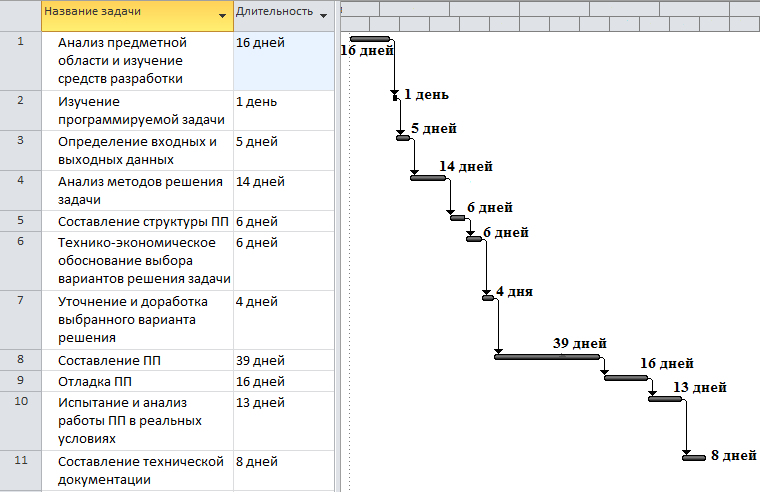
\includegraphics[width=0.9\textwidth, keepaspectratio]{int_op_schedule}
\caption{Календарный план-график работ}\label{fig:economics:schedule}
\end{figure}

\section{Выводы}
В экономической части дипломной работы получены следующие значения экономических показателей:

\begin{itemize}
	\item Технический уровень $J_{\text{\sl ТУ}} = 1.48$. Значение этого показателя должно быть больше 1. Полученное значение говорит о высоком техническом уровне разрабатываемого изделия.
	\item Уровень экономической эффективности $\text{\sl Е}_\text{\sl ПП} = 1.71$.
\end{itemize}

На основании показателей экономической эффективности считаем разрабатываемую систему экономически эффективной и внедрение в производство целесообразным.
	\chapter{Охрана труда и окружающей среды}
\section{Анализ условий труда}
\subsection{Обеспечение условий труда в отделе разработки программного обеспечения}
Дипломная работа посвящена разработке системы мониторинга состояния ЛА на основе алгоритмов интеллектуального анализа данных. Разработка производится на персональном компьютере и предполагает длительное пребывание за ним инженера.

Применение персонального компьютера освобождает человека от непроизводительной работы, связанной с обработкой информации, изменяет характер его труда. Однако при этом увеличивается доля умственного и нервно-напряженного труда, возрастает психоэмоциональная нагрузка. При значительной трудовой нагрузке, нерациональной организации работы и неблагоприятных факторах производственной среды быстро снижается работоспособность операторов, уменьшается производительность труда и ухудшается качество работы, может развиться перенапряжение,~а в отдельных случаях возникнуть срыв трудовой деятельности~--- дистресс.

В данном разделе проводится анализ условий труда в отделе разработки информационных систем с целью обеспечения безопасности и удобства, требуемых для работы инженера.

\subsection{Характеристика помещения}
Помещение находится в здании Московского Авиационного Института и представляет собой кафедральную лабораторию со следующими размерами:
\begin{itemize}
	\item длина~6~м;
	\item ширина~4~м;
	\item высота~3.5~м.
\end{itemize}

Площадь: $6\times4 = 24$~м\textsuperscript{2}.

Объём: $6\times4\times3.5 = 84$~м\textsuperscript{3}.

Количество рабочих мест~---~4.

Количество одновременно находящихся в помещении сотрудников не превышает~4 человек.

План помещения приведён на рисунке~\ref{fig:labourprotection:room_plan}.

\begin{figure}[h]
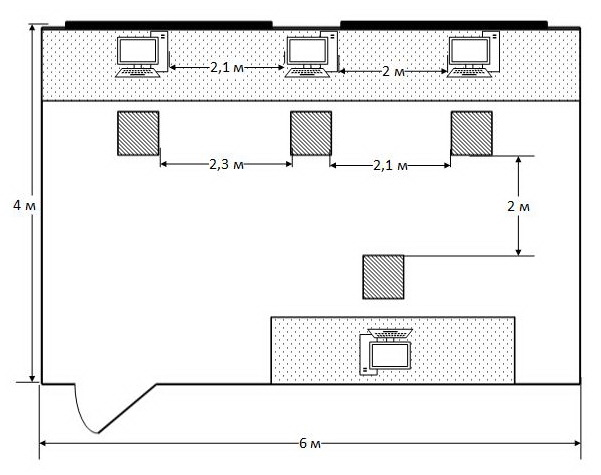
\includegraphics[width=0.6\textwidth, keepaspectratio]{room_plan}
\caption{План помещения}\label{fig:labourprotection:room_plan}
\end{figure}

Нормативные требования к площади и объёму рабочих мест определены в \cite{SanPin2_2_2}:
\begin{itemize}
	\item площадь на одно рабочее место с ВДТ или ПЭВМ для взрослых пользователей должна составлять не~менее~6~м\textsuperscript{2};
	\item объём~---~не~менее~20~м\textsuperscript{3}.
\end{itemize}

Фактические значения на каждого сотрудника:
\begin{itemize}
	\item площадь: $24/4 = 6$~м\textsuperscript{2};
	\item объём: $84/4 = 21$~м\textsuperscript{3}.
\end{itemize}

Данные значения показывают, что кафедральная лаборатория полностью соответствует установленным нормам.

В помещении имеются 2 оконных проёма высотой 1,6~м и шириной 2,3~м, которые выходят на юго-запад.

Искусственное освещение представляет собой 6~светильников, расположенных параллельно окнам в~2~ряда.

\subsection{Характеристика производственного процесса}
Разработка программного обеспечения производится на ПЭВМ с подключенными к ней периферийными устройствами.

\subsection{Характеристика используемого оборудования}
В процессе разработки используется следующее оборудование:
\begin{enumerate}
	\item{ПЭВМ:}
		\begin{enumerate}
			\item{процессор Intel Core i5 3,60 ГГц;}
			\item{оперативная память 8 Гб;}
			\item{жёсткий диск 1 Tб;}
			\item{напряжение питания 220 В.}
		\end{enumerate}
	\item{ЖК монитор с диагональю 23 дюйма (58,42) ASUS VX239H:}
		\begin{enumerate}
			\item{частота 75 Гц;}
			\item{яркость 250 кд/м\textsuperscript{2};}
			\item{динамическая контрастность 8 000 000 : 1;}
			\item{напряжение питания 220 В.}
		\end{enumerate}
	\item{Клавиатура Logitech K330;}
	\item{Мышь A7Tech X;}
	\item{Принтер HP LaserJet 1005M:}
		\begin{enumerate}
			\item{напряжение питания 220 В.}
		\end{enumerate}
\end{enumerate}

\subsection{Санитарно-гигиенические факторы}

\subsubsection{Микроклимат помещения}
Микроклимат в рабочем помещении должен соответствовать \cite{GOST12_1_005}.

Согласно \cite{GOST12_1_005}, работа разработчика ПО относится к категории «Легкая~–~Iа», т.к. лёгкие физические работы~--- работы с расходом энергии не более 150 ккал (174 Вт), а категория Iа подразумевает энергозатраты до 120~ккал/ч~(139 Вт).

Рабочее место разработчика ПО является постоянным, т.к. он находится на нём большую часть рабочего времени (более~50\%).

Нормативные и фактические значения для категории работ «Легкая~–~Iа», лёгкие физические работы~--–~работы с расходом энергии не более 150~ккал (174~Вт). Категория Iа подразумевает энергозатраты до 120~ккал/ч (139~Вт).

Рабочее место разработчика модели является постоянным, т.к. он находится на нём большую часть рабочего времени (более 50\%).

Нормативные и фактические значения для категории работ «Легкая – Iа» и постоянного рабочего места приведены в таблице~\ref{tab:labourprotection:microclimat}.

\begin{table}[h]
\caption{Значения характеристик микроклимата помещения}
\label{tab:labourprotection:microclimat}
\nohyphenation

\begin{tabular}{|C{84pt}|C{178.25pt}|C{101.1pt}|C{110pt}|}
\hline
 & Температура, \textdegree C & Относительная влажность, \% & Скорость движения, м/с \\
\hline
Допустимые значения & 22--24~–-- Холодный период \linebreak 23--25~--– Теплый период & 40--60 & 0.1 \\
\hline
Фактические значения & 22--24~–-- Холодный период \linebreak 25--30~--– Теплый период & 45--55 & <0.1 \\
\hline
\end{tabular}
\end{table}

Фактические значения параметров микроклимата данного помещения удовлетворяют допустимым значениям для холодного периода года. Во время теплого периода в помещении может преобладать повышенная температура из-за отсутствия кондиционера, который бы мог её регулировать.

\subsubsection{Производственное освещение}
Освещённость регламентируется~\cite{SNiP23_05_95}.

Наименьший размер объекта различения в работе инженера составляет 0.3 мм. Объектом является символ, выводимый на экран монитора (наименьшим символом является точка). Зрительная работа относится к III разряду --- высокая точность (наименьший размер объекта различения от 0.3 до 0.5~мм).

Контраст объекта с фоном средний, фон светлый, что соответствует подразряду~б разряда III.

Требования к освещению помещений промышленных предприятий для подразряда~б разряда III:
\begin{itemize}
	\item При системе комбинированного освещения освещенность равна: всего --- 1000 лк, в т.ч. от общего --- 200 лк;
	\item При системе общего освещения освещённость равна 300 лк.
\end{itemize}

Система освещения в комнате общая, состоящая из 6 потолочных светильников ЛПО 46, в каждом из которых установлены 4 люминесцентные лампы ЛТБ мощностью 20 Вт и световым потоком 1100 лм. Светильники расположены в два ряда параллельно окнам. Фактическая освещенность составляет 275 лк, что полностью удовлетворяет нормативным значениям~\cite{SNiP23_05_95}.

\subsubsection{Шум}
Источники шума в данном помещении: охлаждающие системы ПЭВМ (охлаждение процессоров).

Уровни шума на рабочих местах инженера ПЭВМ должны соответствовать~\cite{GOST12_1_003}.

Допустимые значения уровня шума при проектировании и программировании на рабочих местах в помещениях проектно-конструкторских бюро; расчётчиков, программистов вычислительных машин, в лабораториях для теоретических работ и обработки данных: не более  50 дБА.

Фактические значения уровня шума: не более 45 дБА, что подтверждается расчётами в разделе~\ref{sec:labourprotection:calc}.

Согласно~\cite{GOST12_1_003}, значения уровня шума на рабочем месте удовлетворяют установленным требованиям.

\subsubsection{Электромагнитное излучение}
Во время работы ПЭВМ возникают электромагнитные поля, которые оказывают негативное влияние на организм человека.

Источниками электромагнитных полей на рабочем месте инженера являются системные блоки. Современные корпуса системных блоков ПЭВМ позволяют значительно ослабить излучения его элементов. Благодаря существующим достаточно строгим стандартам дозы рентгеновского излучения от современных мониторов и системных блоков не опасны для пользователей.

Документом, регламентирующим уровень электромагнитного излучения для ПЭВМ, является~\cite{SanPin2_2_2}.

Согласно ему, напряжённости электрических и магнитных полей, энергетической нагрузки в течение рабочего дня не должны превышать значений, указанных в таблице~\ref{tab:labourprotection:emradiation}.

\begin{table}[h]
\caption{Предельные значения электромагнитного излучения.}
\label{tab:labourprotection:emradiation}
\nohyphenation

\begin{tabular}{|C{213.35pt}|C{87.35pt}|C{84.4pt}|C{83.4pt}|}
\hline
\multirow{2}{\hsize}{\centering{Параметр}} & \multicolumn{3}{C{255.15pt}|}{Предельные значения в диапазонах частот, МГц} \\
\cline{2-4}
 & от 0.06 до 3 & св. 3 до 30 & св. 30 до 300 \\
\hline
$\text{Е}_\text{ПД}, \text{В/м}$ & 500 & 300 & 80 \\
\hline
$\text{Н}_\text{ПД}, \text{А/м}$ & 50 & --- & --- \\
\hline
$\text{ЭН}_{\text{Е}_\text{ПД}}, \text{(В/м)}^2 \cdot \text{ч}$ & 20000 & 7000 & 800 \\
\hline
$\text{ЭН}_{\text{Н}_\text{ПД}}, \text{(А/м)}^2 \cdot \text{ч}$ & 200 & --- & --- \\
\hline
\end{tabular}
\end{table}

Монитор ASUS VX239H соответствует стандарту~\cite{TCO03}, который устанавливает следующие предельные значения электромагнитного излучения:
\begin{itemize}
	\item напряжённость электрического поля: в диапазоне 5Гц--2кГц не более 10~В/м, в диапазоне 2кГц--400кГц не более 1.0~В/м;
	\item напряжённость магнитного поля: в диапазоне 5Гц--2кГц не более 200~нТл, в диапазоне 2кГц--400кГц не более 25~нТл.
\end{itemize}

Данные характеристики полностью соответствуют требованиям~\cite{SanPin2_2_2}.

\subsection{Электроопасность}
В данном помещении используется оборудование, питающееся от сети переменного тока напряжением 220~В, частотой 50~Гц. 

Согласно~\cite{PUE7}, помещение отдела разработки ИС относится к классу помещений без повышенной опасности поражения электрическим током: это сухое помещение с непроводящими полами, с нормальной температурой воздуха и влажностью, в нем отсутствует токопроводящая пыль.

Электрооборудование в помещении представлено мониторами и системными блоками ПЭВМ. Источником электрического поражения может быть металлический корпус системного блока при пробое изоляции, т.к. имеется напряжение 220~В, а в~\cite{GOST12_1_038} допустимое напряжение и ток для аварийных режимов при времени воздействия более 1~секунды составляют 20~В и 6~мА.

\subsection{Пожароопасность}
В данном помещении имеются твердые горючие и  трудногорючие веще-ства и материалы (книги, документы, деревянная мебель, оргтехника и т.д.), которые при взаимодействии с огнем будут гореть без взрыва. Также источником возгорания может быть электрическая проводка.

Согласно~\cite{GOST12_1_004}, данное помещение относится к классу Б и является пожароопасным.

\subsection{Эргономические факторы}
Требования к организации рабочих мест пользователей ПЭВМ изложены в~\cite{SanPin2_2_2}. 

Согласно~\cite{SanPin2_2_2}, расстояние между рабочими столами с мониторами (в направлении тыла поверхности одного монитора и экрана другого монитора) должно быть не менее 2~м, а расстояние между боковыми поверхностями мониторов не менее 1.2~м.

Фактические значения (см. рисунок~\ref{fig:labourprotection:room_plan}):
\begin{itemize}
	\item расстояние между рабочими столами 2.1--2.5~м;
	\item расстояние между боковыми поверхностями мониторов 2.1-2.3~м.
\end{itemize}

Таким образом, размещение рабочих столов полностью соответствуют требованиям~\cite{SanPin2_2_2}.

В помещении используется специальный стол~--– рабочая поверхность, изготовленная на заказ по выбранным заказчиком параметрам. Ее характеристики и нормативные значения указаны в таблице~\ref{tab:labourprotection:desktop}.

\begin{table}[h]
\caption{Характеристики используемого рабочего стола}
\label{tab:labourprotection:desktop}
\nohyphenation

\begin{tabular}{|C{225.9pt}|C{125.05pt}|C{114.85pt}|}
\hline
Наименование параметра & Нормативное значение~\cite{SanPin2_2_2}, мм & Фактическое значение, мм \\
\hline
Ширина рабочей поверхности & не менее 500  & 1200--2000 \\
\hline
Глубина рабочей поверхности & не менее 800 & 800 \\
\hline
Высота рабочей поверхности & не менее 725 & 800 \\
\hline
Пространство для ног высотой & не менее 600 & 600 \\
\hline
Глубина на уровне колен & не менее 450 & 450 \\
\hline
Глубина на уровне вытянутых ног & не менее 650 & 650 \\
\hline
\end{tabular}
\end{table}

Параметры стола полностью соответствуют требованиям~\cite{SanPin2_2_2}.

В помещении используется офисное кресло БЮРОКРАТ Ch-G318AXN. Его характеристики и нормативные размеры указаны в таблице~\ref{tab:labourprotection:chair}.

%\begin{table}[h]
\begin{longtable}{|C{197.55pt}|C{153.4pt}|C{114.85pt}|}
\caption{Характеристики используемого офисного кресла}
\label{tab:labourprotection:chair}
\\ \hline
Наименование параметра & Нормативное значение~\cite{SanPin2_2_2} & Фактическое значение \\ \hline
\endfirsthead
\LTcontcaption{tab:labourprotection:chair}
\\ \hline
Наименование параметра & Нормативное значение~\cite{SanPin2_2_2} & Фактическое значение \\ \hline
\endhead

Ширина и глубина поверхности сиденья & не менее 400 мм & 420 мм \\
\hline
Регулировка высоты поверхности сиденья  & 400--550 мм & 440--570 мм \\
\hline
Регулировка углов наклона сиденья & вперед до 15\textdegree и назад до 5\textdegree & вперед до 15\textdegree и назад до 5\textdegree \\
\hline
Высота опорной поверхности спинки & 300 ± 20 мм & 310 мм \\
\hline
Ширина опорной поверхности спинки & не менее 380 мм & 380 мм \\
\hline
Радиус кривизны горизонтальной плоскости опорной поверхности спинки & 400 мм & 400 мм \\
\hline
Угол наклона спинки в вертикальной плоскости & ± 30\textdegree & ± 30\textdegree \\
\hline
Регулировка расстояния спинки от переднего края сиденья & 260--400 мм & 260--450 мм \\
\hline
Стационарные или съёмные подлокотники & длина не менее 250 мм \linebreak ширина 50--70 мм & длина 250 мм \linebreak ширина 60 мм \\
\hline
Регулировка подлокотников по высоте над сиденьем & 230 ± 30 мм & Нет \\
\hline
Регулировка внутреннего расстояния между подлокотниками & 350--500 мм & 420--500 мм \\
\hline
\end{longtable}
%\end{table}

Параметры стула частично не соответствуют требованиям \cite{SanPin2_2_2}: в данном рабочем кресле отсутствует регулировка подлокотников по высоте над сидением.

\subsection{Психофизиологические факторы}
Факторами, оказывающими влияние на внимательность инженера и его производительность труда, в условиях его рабочего места являются:
\begin{itemize}
	\item визуальные характеристики монитора (его яркость, контрастность, разрешение, частота обновления); 
	\item напряженность работы; 
	\item количество обрабатываемой информации –-- плотность воспринимаемых сигналов.
\end{itemize}

Используется ЖК монитор ASUS VX239H. Его фактические характеристики и нормативные значения~\cite{SanPin2_2_2} приведены в таблице~\ref{tab:labourprotection:display}.

\begin{table}[h]
\caption{Характеристики используемого ЖК монитора}
\label{tab:labourprotection:display}
\nohyphenation

\begin{tabular}{|C{178.9pt}|C{152.25pt}|C{158.9pt}|}
\hline
Наименование фактора & Действительное значение & Нормативное значение~\cite{SanPin2_2_2} \\
\hline
Размер экрана по диагонали & 58,42 см & не менее 31 см \\
\hline
Удалённость экрана & 60 см & не менее 50 см \\
\hline
Частота обновления изображения & 75 Гц & не менее 75 Гц \\
\hline
Контрастность & 8 000 000:1 & не менее 3:1 \\
\hline
Яркость знака & 250 кд/м2 & не менее 35 кд/м2 \\
\hline
\end{tabular}
\end{table}

Характеристики монитора полностью соответствуют требованиям~\cite{SanPin2_2_2}.

Напряженность работы на основании данных таблицы классов условий труда по показателям напряженности трудового процесса \cite{R2_2_2006} представлена в таблице~\ref{tab:labourprotection:workintensity}.

\begin{longtable}{|C{165pt}|C{165pt}|C{160pt}|}
\caption{Напряженность работы}
\label{tab:labourprotection:workintensity}
\\ \hline
Критерий & Характеристика & Напряженность трудового процесса \\ \hline
\endfirsthead
\LTcontcaption{tab:labourprotection:workintensity}
\\ \hline
Критерий & Характеристика & Напряженность трудового процесса \\ \hline
\endhead

Содержание работы & Решение сложных задач по известным алгоритмам (работа по серии инструкций) & Напряженный труд 1 степени \\
\hline
Восприятие сигналов (информации и их оценка) & Восприятие сигналов с последующей комплексной оценкой взаимосвязанных параметров & Напряженный труд 2 степени \\
\hline
Степень сложности задания & Обработка, проверка и контроль за выполнением задания & Напряженность труда средней степени \\
\hline
Характер выполняемой работы & График с возможной корректировкой & То же \\
\hline
Длительность сосредоточенного наблюдения (в \% от времени смены) & 26--50\% & --//-- \\
\hline
Плотность сигнала за 1 час работы & 176--300 & Напряженный труд 1 степени \\
\hline
Число объектов одновременного наблюдения & 6--10 & Напряженность труда средней степени \\
\hline
Размер объекта различения, мм, при длительном сосредоточенном наблюдении (\% времени смены) & 3--10 мм до 50\% времени & То же \\
\hline
Степень ответственности & Ответственность за качество конечного результата & Напряженный труд 2 степени \\
\hline
Значимость ошибки & Влечет за собой дополнительные усилия в работе со стороны работника & Напряженность труда лёгкой степени \\
\hline
Продолжительность рабочего дня & 8--9 часов & Напряженность труда средней степени \\
\hline
\end{longtable}

Среднее значение по данным критериям соответствует средней степени напряженности труда.

\section{Мероприятия по обеспечению условий труда}
Микроклимат в помещении в холодное время года обеспечивается с помощью системы центрального отопления. В летний же период времени в помещении не происходит регулирования температуры и влажности из-за отсутствия кондиционера. Рекомендуется установить, например, потолочный кондиционер Panasonic CS-A18BTP/CU-A18BBP5 с циркуляцией воздуха 840~м\textsuperscript{3}/час.

Мероприятия по обеспечению требуемых условий по освещенности можно отнести к выбору ламп в источниках света. Часть цвет предметов освещенных люминесцентными лампами может быть несколько искажён и быть неприятен человеку. Это, в свою очередь, вызывает усталость и напряженность глаз. Для предотвращения этого целесообразно использовать лампы с «трехполосным» и «пятиполосным» люминофором~--- веществом, способным преобразовывать поглощаемую им энергию в световое излучение. Это позволяет добиться более равномерного распределения излучения по видимому спектру, что приводит к более натуральному воспроизведению света. Данным параметрам соответствует лампа Philips Master~TL-D De~Luxe~36W/D65.

Уровень шума при использовании описанных ПЭВМ не превосходит норм, поэтому дополнительных мер для предотвращения излишнего шума не требуется. При закупке нового оборудования следует учитывать уровень шума от каждой новой единицы.

Обеспечение электробезопасности основано на применении устройств защитного отключения (УЗО). Данное устройство реагирует на ухудшение изоляции электропроводки: когда ток утечки повысится до предельной величины 30 мА, происходит отключение напряжения в течение 30 микросекунд. Целесообразно применять УЗО Legrand DX~06576.

Пожаробезопасность должна быть обеспечена при помощи обработки жидкостью от возгорания предметов мебели, инструктажа персонала на предмет мер предотвращения пожара или эвакуационных действий при пожаре, тщательной проверки оборудования на предмет повреждения проводов или оборудования.

\section{Расчетная часть}\label{sec:labourprotection:calc}
\subsection{Расчет уровня шума}
Цель расчета~–-- определить, соответствует ли фактический уровень шума в помещении нормативным значениям. Основными источниками шума в рассматриваемом помещении является аппаратура системных блоков ПЭВМ (кулер процессора).

Расчет производится в соответствии с~\cite{LabourProtOnCC}.

План помещения с указанием рабочих мест и рабочей точки показан на рисунке~\ref{fig:labourprotection:room_plan_wp}

\begin{figure}[h]
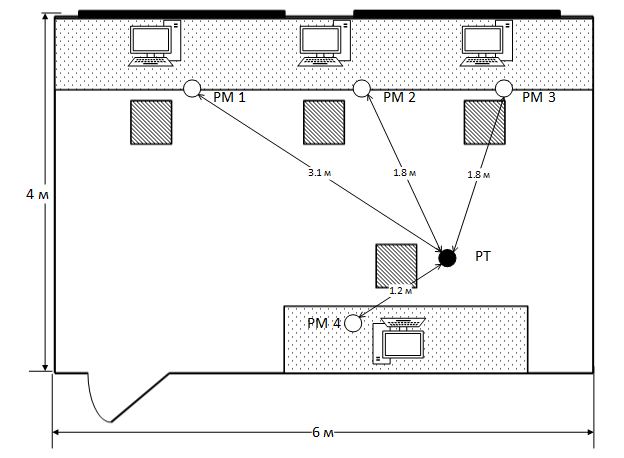
\includegraphics[width=0.67\textwidth, keepaspectratio]{room_plan_wp}
\caption{План помещения с указанием рабочих мест и рабочей точки}\label{fig:labourprotection:room_plan_wp}
\end{figure}

Будем считать, что оператор, находящийся в расчётной точке,  располагается в зоне действия прямого звука. Тогда фактические значения уровней звукового давления в октановых полосах частот на расстоянии $r$ от источника и суммарных значений от нескольких источников рассчитываются по формулам~\ref{eq:labourprotection:noise}~и~\ref{eq:labourprotection:noisesum}.

\begin{equation}\label{eq:labourprotection:noise}
L_i = L_{W_i} - 20 \cdot \log{r_i} - 11 \text{;}
\end{equation}
\begin{equation}\label{eq:labourprotection:noisesum}
L_{\sum} = 10 \cdot \log{\sum_{i=1}^{n} 10^{0.1 \cdot L_i}} \text{,}
\end{equation}
\begin{description}
	\item[где $L_{W_i}$] --- уровень звуковой мощности $i$-го источника.
\end{description}
\smallskip

Допустимые уровни звукового давления в расчётной точке представлены в соответствии с~\cite{SanPin2_2_2}.

Расстояния от рабочих мест до рабочей точки:

\smallskip
$r_1 = 1.8 \text{м}, r_2 = 1.8 \text{м}, r_3 = 3.1 \text{м}, r_4 = 1.2 \text{м}.$
\smallskip

Уровни звукового давления для источников шума 1-4 (РМ1-РМ4) для уровня звуковой мощности кулера $L = 38 \text{ дБ}$ и среднегеометрической частоты 500 Гц:

\smallskip
$\begin{aligned}
L_1 = 38 - 20 \cdot \log{1.8} - 11 = 31.9 \text{ дБ;}\\
L_2 = 38 - 20 \cdot \log{1.8} - 11 = 31.9 \text{ дБ;}\\
L_3 = 38 - 20 \cdot \log{3.1} - 11 = 27.2 \text{ дБ;}\\
L_4 = 38 - 20 \cdot \log{1.2} - 11 = 38.5 \text{ дБ.}\\
\end{aligned}$
\smallskip

В этом случае уровень звукового давления от 4 источников:

\smallskip
$L_{\sum} = 10 \cdot \log(10^{0.1 \cdot 31.9} + \log(10^{0.1 \cdot 31.9} + \log(10^{0.1 \cdot 27.2} + \log(10^{0.1 \cdot 38.5}) = 38.5 \text{ дБ.}$
\smallskip

Уровни звукового давления для источников шума 1-4 (РМ1-РМ4) для уровня звуковой мощности кулера $L = 37 \text{ дБ}$ и среднегеометрической частоты 1000 Гц:

\smallskip
$\begin{aligned}
L_1 = 37 - 20 \cdot \log{1.8} - 11 = 30.9 \text{ дБ;}\\
L_2 = 37 - 20 \cdot \log{1.8} - 11 = 30.9 \text{ дБ;}\\
L_3 = 37 - 20 \cdot \log{3.1} - 11 = 26.2 \text{ дБ;}\\
L_4 = 37 - 20 \cdot \log{1.2} - 11 = 37.5 \text{ дБ.}\\
\end{aligned}$
\smallskip

В этом случае уровень звукового давления от 4 источников:

\smallskip
$L_{\sum} = 10 \cdot \log(10^{0.1 \cdot 30.9} + \log(10^{0.1 \cdot 30.9} + \log(10^{0.1 \cdot 26.2} + \log(10^{0.1 \cdot 37.5}) = 37.5 \text{ дБ.}$
\smallskip

Уровни звукового давления источников шума для остальных частот рассчитываются аналогично. Результаты расчётов сведены в таблицу~\ref{tab:labourprotection:calcresults}.

\begin{table}[h]
\caption{Сводная таблица значений уровней шума}
\label{tab:labourprotection:calcresults}
\nohyphenation

\begin{tabular}{|C{160pt}|C{32pt}|C{32pt}|C{32pt}|C{32pt}|C{32pt}|C{32pt}|C{32pt}|C{32pt}|}
\hline
Среднегеометрическая частота, Гц & 63 & 125 & 250 & 500 & 1000 & 2000 & 4000 & 8000 \\
\hline
Уровень звуковой мощности кулера блока питания, дБ & 35 & 37,5 & 37,5 & 38 & 37 & 36,5 & 36,5 & 35,5 \\
\hline
Уровень звукового давления от источника шума 1 (РМ1) при r = 1.8 м, дБ & 28.9 & 31.4 & 31.4 & 31.9 & 30.9 & 30.4 & 30.4 & 29.4 \\
\hline
Уровень звукового давления от источника шума 2 (РМ2) при r = 1.8 м, дБ & 28.9 & 31.4 & 31.4 & 31.9 & 30.9 & 30.4 & 30.4 & 29.4 \\
\hline
Уровень звукового давления от источника шума 3 (РМ3) при r = 3.1 м, дБ & 24.2 & 26.7 & 26.7 & 27.2 & 26.2 & 25.7 & 25.7 & 24.7 \\
\hline
Уровень звукового давления от источника шума 4 (РМ4) при r = 1.2 м, дБ & 32.4 & 34.9 & 34.9 & 35.4 & 34.4 & 33.9 & 33.9 & 32.9 \\
\hline
Уровень звукового давления от 4 источников шума, дБ & 35.5 & 38 & 38 & 38.5 & 37.5 & 37 & 37 & 36 \\
\hline
Допустимый уровень звукового давления в расчетной точке (РТ), дБ & 71 & 61 & 54 & 49 & 45 & 42 & 40 & 38 \\
\hline
\end{tabular}
\end{table}

Уровень шума в расчетной точке не превышает допустимые значения, таким образом, не требуются никакие мероприятия по снижению шума в помещении.
%\FloatBarrier

\section{Вывод}
В разделе «Охрана труда и окружающей среды» был проведен анализ условий труда инженера-программиста по следующим факторам: санитарно-гигиеническим, эргономическим, психофизическим; была проведена оценка помещения по электроопасности и пожароопасности. Также были предложены мероприятия по обеспечению требований предъявляемых к эргономическим характеристикам рабочего места. В расчетной части был осуществлен расчет уровня шума в помещении, в результате которого были получены значения, не превышающие допустимые.
 
По всем перечисленным факторам было выявлено соответствие нормам и требованиям ГОСТов, СанПиНов и СНиПу.
	\spchapter{Заключение}
В рамках дипломной работы были выполнены следующие пункты:
\begin{itemize} 
	\item произведён анализ существующих алгоритмов выявления аномалий без учителя, выделены их достоинства и недостатки;
	\item создан метод мониторинга состояния ЛА на основе алгоритмов интеллектуального анализа данных, устраняющий недостатки существующих методов;
	\item разработана его программная реализация.
\end{itemize}

В результате разработки все требования задания были полностью удовлетворены. Разработанная программная реализация метода позволет строить модель произвольной системы для последующего контроля и диагностики её состояния только на основе данных телеметрии при различных режимах её работы, без априорных знаний о предметной области, назначении системы, её составе, конструкции. Система обладает способностью обучаться на больших массивах исходных данных, учитывает как дискретные, так и непрерывные параметры, устойчива к аномалиями в обучающих выборках и может осуществлять контроль даже при отсутствии некоторых параметров в измерениях. Разработанное ПО обладает достаточным быстродействием для работы в режиме реального времени.

Результаты проведённого тестирования свидетельствуют об отсутствии ошибок контроля в работе системы и показывают её соответствие заявленным характеристикам.

Система может применяться для своевременного контроля состояния ЛА научно-измерительными пунктами (НИП) на основе данных телеметрии. Разработанный метод может быть реализован в качестве бортовой системы мониторинга, но это исследование выходит за рамки данной дипломной работы.

В экономической части дипломной работы была проведена оценка экономической эффективности разработанного ПО, которая показала, что внедрение разработанной системы в эксплуатацию является целесообразным.

В разделе «Охрана труда и окружающей среды» был проведен анализ условий труда при разработке программного обеспечения. Также был рассчитан уровень шума в помещении, позволяющий обеспечить комфортные условия труда и повысить его производительность, а также даны рекомендации по обеспечению условий труда в соответствии с принятыми нормами и ГОСТами.
	
	\addcontentsline{toc}{chapter}{\bibname}
	\nocite{*}
	\bibliography{thesis}
	
	\appendix
	\begin{appendices}
		\chapter{Исходный код}
\begin{algorithm}
\caption{Псевдкод алгоритма Orca}
\begin{algorithmic}[1]
\REQUIRE $n \geq 0$
\ENSURE $y = x^n$
\STATE $y \leftarrow 1$
\STATE $X \leftarrow x$
\STATE $N \leftarrow n$
\WHILE{$N \neq 0$}
\IF{$N$ is even}
\STATE $X \leftarrow X \times X$
\STATE $N \leftarrow N / 2$
\ELSE[$N$ is odd]
\STATE $y \leftarrow y \times X$
\STATE $N \leftarrow N - 1$
\ENDIF
\ENDWHILE
\end{algorithmic}
\end{algorithm}

\begin{lstlisting}
foreach (var x in values)
{
	int i = x.Key;
	Console.WriteLine("Key: {0}", i);
}
\end{lstlisting}
		\chapter{Графические материалы}
*тут должны быть слайды*
	\end{appendices}
\end{document}